\documentclass[leqno,labelfig,psfigt,colorlinks]{svmono}

%\usepackage[a4paper,left=1cm,right=10cm,bindingoffset=5pt, asymmetric, reversemarginpar]{geometry}

\makeatletter
\providecommand*{\input@path}{}
\edef\input@path{{./}{../}\input@path}% prepend
\makeatother

%% Macros for AMG notes
%\newcommand{\triplenorm}[1]{\ensuremath{| \! | \! | #1 | \! | \! |}}
\newcommand{\triplenorm}[1]{%
  \left\vert\kern-0.9pt\left\vert\kern-0.9pt\left\vert #1
  \right\vert\kern-0.9pt\right\vert\kern-0.9pt\right\vert}
\newcommand{\Tscalar}[2]{\ensuremath{(#1 , #2)_{\bar R^{-1}}}} %%% macro for star norm.
\newcommand{\Tnorm}[1]{\ensuremath{\|#1\|_{\bar R^{-1}}}}
\newcommand{\Dscalar}[2]{\ensuremath{( #1 , #2 )_D}}
\newcommand{\Dnorm}[1]{\|#1\|_{D}}
\newcommand{\Tproj}{\ensuremath{Q_c}}
\newcommand{\Dproj}{\ensuremath{Q_D}}
\newcommand{\Anorm}[1]{\|#1\|_A}
\newcommand{\trace}{\ensuremath{\operatorname{trace}}}
\newcommand{\Span}{\ensuremath{\operatorname{span}}}

\newcommand{\eqqsim}{\mathbin{\rotatebox[origin=c]{180}{\ensuremath{\cong}}}}

\newcommand{\rs}{\ensuremath{R_s}}

\newcommand{\Vhf}{V_{\rm hf}}
\newcommand{\Vf}{V_{f}}
\newcommand{\Vc}{V_{c}}
\newcommand{\sparse}{\ensuremath{\operatorname{S}}}
\newcommand{\dof}{\ensuremath{N}}
\newcommand{\co}{\ensuremath{C_{o}}}
\newcommand{\Nepo}{{Nepomnyaschikh}}
\renewcommand{\v}{{\cal V}}
% ---------------------------
% packages
% ---------------------------
% AMS math symbol
\usepackage{amsmath}
\usepackage{amsbsy}
\usepackage{amsfonts}
\usepackage{amssymb}
\usepackage{amscd}
\usepackage{mathrsfs}
%\usepackage{mathptmx}       % selects Times Roman as basic font
%\usepackage{algorithmic}
\usepackage{bm}
%\usepackage{wsuipa}

\usepackage{algpseudocode}
\usepackage[Algorithm]{algorithm}
%% one line ifs and fors commands only for this section
\algnewcommand{\IIf}[1]{\State\algorithmicif\ #1\ \algorithmicthen}
\algnewcommand{\EElse}{\unskip\ \algorithmicelse\ }
\algnewcommand{\EndIIf}{\unskip\ \algorithmicend\ \algorithmicif}
\algnewcommand{\FFor}[1]{\State\algorithmicfor\ #1\ }
\algnewcommand{\EndFFor}{\unskip\ \algorithmicend\ \algorithmicfor}
%%%%%%%%%%%%%%%%%%%%%%%%%%%%%%%%%%%%%

% text fonts
\usepackage{txfonts}
%\usepackage{helvet}         % selects Helvetica as sans-serif font
%\usepackage{courier}        % selects Courier as typewriter font
\usepackage[latin1]{inputenc}

% graphcis
\usepackage{graphicx}
\usepackage{subfigure} %commented by Ludmil, uncommented by Hongxuan
\usepackage{float}

\usepackage{tikz}   %commented by Ludmil, uncommented by Hongxuan
\usetikzlibrary{shapes,arrows,decorations.pathmorphing,backgrounds,positioning,fit,matrix,calc}  %commented by Ludmil, uncommented by Hongxuan
%\usepackage{subfig}  %added by Ludmil, commented by Hongxuan

\tikzstyle{decision} = [diamond, draw, fill=blue!20,
    text width=4.5em, text badly centered, node distance=3cm, inner sep=0pt]
\tikzstyle{block} = [rectangle, draw, fill=blue!20,
    text width=5em, text centered, rounded corners, minimum height=4em]
\tikzstyle{line} = [draw, -latex']
\tikzstyle{cloud} = [draw, ellipse,fill=red!20, node distance=3cm,
    minimum height=2em]



%% command shell environment 
\usepackage[most]{tcolorbox}
\newtcblisting{commandshell}{colback=black,colupper=white,colframe=yellow!75!black,
listing only,listing options={language=sh},
every listing line={\textcolor{red}{\small\ttfamily\bfseries Terminal \$> }}}

%% Code styles
\usepackage{listings}
\usepackage{color}
 
\definecolor{codegreen}{rgb}{0,0.6,0}
\definecolor{codegray}{rgb}{0.5,0.5,0.5}
\definecolor{codepurple}{rgb}{0.58,0,0.82}
\definecolor{backcolour}{rgb}{0.95,0.95,0.92}
 
\lstdefinestyle{python}{
    backgroundcolor=\color{backcolour},   
    commentstyle=\color{codegreen},
    keywordstyle=\color{magenta},
    numberstyle=\tiny\color{codegray},
    stringstyle=\color{codepurple},
    basicstyle=\footnotesize,
    breakatwhitespace=false,         
    breaklines=true,                 
    captionpos=b,                    
    keepspaces=true,                 
    numbers=left,                    
    numbersep=5pt,                  
    showspaces=false,                
    showstringspaces=false,
    showtabs=false,                  
    tabsize=2
}
 
%\lstset{style=python}


% other tools
\usepackage{hyperref}
\usepackage{type1cm}
%%\usepackage[normalem]{ulem}
\usepackage{soul}
%\usepackage{times}
\usepackage{url}
\usepackage{undertilde}
%\usepackage{ulem}
%\def\utilde{\uwave}
\usepackage{rotating} %% commented because it crashes "figure" (ludmil), uncommented by Hongxuan
\usepackage{makeidx}
\makeindex             % used for the subject index
\usepackage{multicol}
\usepackage{enumerate}
\usepackage{xspace}
 \usepackage{comment}  % added by Ludmil
 % \usepackage[bw,framed]{mcode} %% commented because it crashes "lstlisting" (ludmil)
\usepackage[margins]{trackchanges} %% commented because it crashes "figure" (ludmil), uncommented by Hongxuan
\usepackage{etoolbox}
\usepackage{array}
%%
% ---------------------------
% Formats
% ---------------------------
% head
\usepackage{fancyhdr}
\pagestyle{fancy}
\rhead{} %added by Hongxuan Zhang

% page
\pagenumbering{arabic}
\newcommand{\pinput}[1]
{\newpag
\hrule
\centerline{\huge \bf #1}
\hrule
\newpage}

% ---------------------------
% Theorems etc.
% ---------------------------
\ifcsmacro{theorem}{}{
\newtheorem{theorem}{Theorem}[section]
}
\ifcsmacro{lemma}{}{
\newtheorem{lemma}[theorem]{Lemma}
}
\ifcsmacro{corollary}{}{
\newtheorem{corollary}[theorem]{Corollary}
}
\ifcsmacro{proposition}{}{
\newtheorem{proposition}[theorem]{Proposition}
}
\ifcsmacro{algorithm}{}{
\newtheorem{algorithm}[equation]{Algorithm}
}
\newtheorem{consequence}[equation]{Consequence}
\newtheorem{conclusion}[equation]{Conclusion}
\newcommand{\Remark}{\noindent{\bf Remark.~}}
\newtheorem{assumption}[equation]{Assumption}
\newtheorem{observation}[equation]{Observation}
%\newtheorem{remark}[theorem]{Remark}
%\newtheorem{definition}[theorem]{Definition}
%\newtheorem{exercise}[theorem]{Exercise}
\newtheorem{homework}[theorem]{Homework}
%\newtheorem{example}[theorem]{Example}

\def\proof{\par{\it Proof}. \ignorespaces}
\def\endproof{{\ \vbox{\hrule\hbox{\vrule
        height1.3ex\hskip0.8ex\vrule}\hrule}}\par}

% ---------------------------
% Chapter and sections
% ---------------------------
\let\oldchapter\chapter
\def\chapter{%
  \setcounter{exercise}{0}%
  \oldchapter
}

% ---------------------------
% New commands
% ---------------------------
% References and Citation
%\newcommand{\Label}[1]{\label{#1}{{\mbox{\small\mbox{\fbox{\tt #1}\quad}}}}}
\newcommand{\Label}{\label}
\newcommand{\Rf}[1]{\mbox{$(\ref{#1})$}}
\newcommand{\rf}[1]{$(\ref{#1})$}

\DeclareMathOperator*{\argmin}{arg\,min}
\DeclareMathOperator*{\argmax}{arg\,max}
\DeclareMathOperator*{\range}{Range}
%\DeclareMathOperator*{\span}{span}

% making comment
% \renewcommand{\initialsOne}{Xu}
% \renewcommand{\initialsTwo}{XHu}
% \renewcommand{\initialsThree}{Yang}
% \renewcommand{\initialsFour}{Zhang}
% \renewcommand{\initialsFive}{KHu}


%\newcommand{\sh}{{\cal S}_h}
% new math command
\newcommand{\pro}{{\mathcal P}}
\newcommand{\beas}{\begin{eqnarray*}}
\newcommand{\eeas}{\end{eqnarray*}}
\newcommand{\bary}{\begin{array}}
\newcommand{\eary}{\end{array}}
\newcommand{\supp}{{\rm supp}\;}
\newcommand{\update}{\leftarrow}
\newcommand{\cequiv}{\stackrel{\mathrm{c}}{\equiv}}
\newcommand{\hf}{\frac{1}{2}}
\newcommand{\qall}{\quad\forall\;}
\def\ec{\mathrel{\hbox{$\copy\Ea\kern-\wd\Ea\raise-3.5pt\hbox{$\sim$}$}}}
\newcommand{\lc}{\mathrel{\raise2pt\hbox{${\mathop<\limits_{\raise1pt\hbox{\mbox{$\sim$}}}}$}}}
\newcommand{\gc}{\mathrel{\raise2pt\hbox{${\mathop>\limits_{\raise1pt\hbox{\mbox{$\sim$}}}}$}}}
\newcommand{\deq}{\stackrel{\rm def}{=}}
\newcommand{\cths}{\{\cth: h\in\aleph\}}
\newcommand{\td}[1]{\tilde{#1}}
\newcommand{\spd}{SPD }
\newcommand{\step}[1]{\noindent\raisebox{1.5pt}[10pt][0pt]{\tiny\framebox{$#1$}}\xspace}
\newcommand{\topic}[1]{\vspace{2mm}\addtocounter{equation}{1}{\noindent{\bf(\theequation) \ {\sf #1}.}}\ }
\newbox\Ea
\setbox\Ea=\hbox{\raise0.9pt\hbox{$=$}}
\newcommand{\smt}[1]{\overline{#1}}%% Notation for matrix, to be modified.
\newcommand{\rep}[1]{{\widetilde {#1}}}%% Notation for matrix representation
\newcommand{\mt}{\mathcal}%% Notation for matrix, to be modified.
\newcommand{\hcomment}[1]{\mbox{\quad (#1)}}
\newcommand{\tol}{\mbox{\rm tol}}
\newcommand{\diag}{\mbox{diag}\;}
\newcommand{\for}{\sf for\mbox{$\;$}}
\newcommand{\efor}{\mbox{\sf endfor}}
\newcommand{\ot}[1]{\mbox{\bf{$#1$}}}
\newcommand{\hset}{{\aleph}}
\newcommand{\thset}{\{{\cal T}_h: h\in \hset\}}
\newcommand{\mbb}{\mathbb}
\newcommand{\bs}{\boldsymbol}
\newcommand{\mcal}{\mathcal}
\newcommand{\mrm}{\mathrm}
\newcommand{\dist}{\mbox{dist}\;}
\newcommand{\prt}[1]{\frac{\partial}{\partial #1}}
\newcommand{\prtt}[2]{\frac{\partial #1}{\partial #2}}
\newcommand*{\ang}[1]{\left\langle #1 \right\rangle}
\newcommand{\bproof}{\begin{proof}}
\newcommand{\eproof}{\end{proof}}

% new letters
\newcommand{\nne}{\mbox{$n_{\mbox{\tiny E}}$}}
\newcommand{\At}{\mbox{$A_{\mbox{\tiny T}}$}}
\newcommand{\rhst}{\mbox{${f}_{\mbox{\tiny T}}$}}
\newcommand{\rhs}{\mbox{$f$}}
\newcommand{\nt}{\mbox{$NT$}}
\newcommand{\ib}{\mbox{$IB$}}
\newcommand{\nn}{\mbox{$n$}}
\newcommand{\om}{\Omega}  % needs to get rid of it
\newcommand{\Om}{\Omega}
\newcommand{\cM}{{\cal M}}
\newcommand{\m}{\mbox{$\cM$}}
\newcommand{\cT}{\mbox{${\cal T}$}}
\newcommand{\cP}{{\mathcal P}}
\newcommand{\ct}{{\cal T}}  % need to get rid of it
\newcommand{\cth}{{\cal T}_h}
\newcommand{\Th}{\mbox{${\cal T}_h$}}
\newcommand{\ld}{\lambda}
\newcommand{\nh}{{\cal N}_h}
%%%\renewcommand{\v}{{\cal V}}
\newcommand{\vvv}{{\cal V}}
\newcommand{\vh}{{\cal V}_h}
\newcommand{\newu}{u^{new}}
\newcommand{\oldu}{u^{\rm old}}
\newcommand{\oldr}{r^{\rm old}}
\newcommand{\LL}{L}
\newcommand{\Sh}{{\cal S}^h}
\newcommand{\Shz}{{\cal S}^h_0}
\newcommand{\V}{V}
\newcommand{\Q}{Q}
\newcommand{\Ddivh}{\mbox{\bf A}_h^{\rm div}}
\newcommand{\hb}{\hat B}
\newcommand{\tqk}{\tilde Q_k}
\newcommand{\vaip}{\overline{a}}
\newcommand{\Prol}{\Pi}
\newcommand{\Aa}{\bar A}

% operators
\newcommand{\grad}{{\rm grad}}
\newcommand{\curl}{{\rm curl }}
\newcommand{\dv}{{\rm div}}
\newcommand{\divg}{{\rm div}\mbox{$\;$}}
\newcommand{\Hcurl}{{\rm curl}}
\newcommand{\Hg}{H({\rm grad})}

% projections
\newcommand{\Phz}{\Pi_h^0}
\newcommand{\Phg}{\Pi_h}
\newcommand{\Phd}{\Pi_h^{\rm div}}
\newcommand{\PHdiv}{\Pi_H^{\rm div}}
\newcommand{\Phc}{\Pi_h^{\rm curl}}
\newcommand{\PHc}{\Pi_H^{\rm curl}}
\newcommand{\PHcurl}{\Pi_H^{\rm curl}}
\newcommand{\PHd}{\Pi_H^{\rm div}}
\newcommand{\PHz}{\Pi_H^{\rm 0}}

% inner product, norm
\newcommand{\inner}{\mbox{$(\cdot, \cdot)$}}
\newcommand{\innerA}{(\cdot,\cdot)_A}
\newcommand{\nm}[2]{\|{#1}\|_{#2}}
\newcommand{\nmA}[1]{\nm{#1}{A}}
\newcommand{\NA}[1]{\|#1\|_{A}}
\newcommand{\nmm}[1]{\|#1\|}
\newcommand{\trnm}[2]{|\!\!|\!\!|{#1}|\!\!|\!\!|_{#2}}

% space
\newcommand{\ho}{H^1_0(\Om)}
\ifcsmacro{R}{}{
\newcommand{\R}{\mathbb{R}} %% this does not work as \R^{blah blah} better do not use (--ltz)
}
\newcommand{\Z}{\mathbb{Z}}
%\newcommand\Rn[1]{\R^{#1}}
\newcommand{\Hd}{\mbox{$\ot H({\rm div})$}}
\newcommand{\Hdiv}{\mbox{$\ot H({\rm div})$}}
\newcommand{\Hhdiv}{\mbox{$\ot H_h({\rm div})$}}
\newcommand{\HHdiv}{\mbox{$\ot H_H({\rm div})$}}
\newcommand{\Zdiv}{\mbox{$\ot Z({\rm div})$}}
\newcommand{\Zzdiv}{\mbox{$\ot Z_0({\rm div})$}}
\newcommand{\Zhdiv}{\mbox{$\ot Z_h({\rm div})$}}
\newcommand{\ZHdiv}{\mbox{$\ot Z_H({\rm div})$}}
\newcommand{\Hc}{\mbox{$\ot H({\rm curl})$}}
\newcommand{\Hcllurl}{\mbox{$\ot H({\rm curl})$}}
\newcommand{\Hzcurl}{\mbox{$\ot H_0({\rm curl})$}}
\newcommand{\Hhcurl}{\mbox{$\ot H_h({\rm curl})$}}
\newcommand{\HHcurl}{\mbox{$\ot H_H({\rm curl})$}}
\newcommand{\Hhg}{\mbox{$H^1_h$}}
\newcommand{\Hhd}{\mbox{$H_h^{\rm div}$}}
\newcommand{\Hhc}{\mbox{$H_h^{\rm\small curl}$}}
\newcommand{\Hhz}{\mbox{$L^2_h$}}
\newcommand{\Cinf}{C^\infty}
\newcommand{\cc}{C(\bar \Omega)}
\newcommand{\ccc}{C^{0,\lambda}(\bar \Omega)}
\newcommand{\hoz}{H_0^1(\Om)}
\newcommand{\HHg}{\mbox{$H_H^1$}}
\newcommand{\czi}{C_0^\infty(\Omega)}
\newcommand{\domega}{{\cal D}(\Omega)}
\newcommand{\ddomega}{{\cal D}'(\Omega)}
\newcommand{\nmt}[2]{|\!|\!|#1|\!|\!|_{#2}^{\sim}}
\newcommand{\nmaa}[1]{\|#1\|_{0,(\alpha)}}
\newcommand{\nmg}[2]{\nm{#1}{H^{#2}(\Om)}}
\newcommand{\ucc}{\nm{u}{0,\infty}}
\newcommand{\uccc}{\nm{u}{\ccc}}
\newcommand{\unpp}{\nm{u}{W^{d/p,p}(\Omega)}}
\newcommand{\eps}{\epsilon}
\newcommand{\la}{\langle}
\newcommand{\ra}{\rangle}
\newcommand{\La}{L^{(\alpha)}(\Omega)}
\newcommand{\Ref}[1]{\ref{#1}}
\newcommand{\apprle}{\lesssim}


%%%%%%%%% MULTIGRID FOR H(DIV) AND H(CURL)%%%
\newcommand{\diam}{\mbox{\rm diam\,}}
%\newcommand{\curl}{{\rm\bf  curl}}
%\newcommand{\grad}{{\rm\bf grad}}
%\DeclareMathOperator*{\supp}{supp}
\renewcommand{\div}{{\operatorname{div}}}
\newcommand{\sdiv}{\mbox{{\footnotesize div}}}
\newcommand{\scurl}{\mbox{{\footnotesize curl}}}%\newcommand{\eps}{\varepsilon}

\newcommand{\N}{{\mathbb N}}
%\renewcommand{\P}{{\mathbb{P}}}
%\newcommand{\R}{{\mathbb R}}
%\newcommand{\V}{{\mathbb V}}
\newcommand{\W}{{\mathbb W}}

\newcommand{\cA}{{\mathcal A}}
\newcommand{\cB}{{\mathcal B}}
\newcommand{\cC}{{\mathcal C}}
\newcommand{\cD}{{\mathcal D}}
\newcommand{\cE}{{\mathcal E}}
\newcommand{\cF}{{\mathcal F}}
\newcommand{\cH}{{\mathcal H}}
\newcommand{\cI}{{\mathcal I}}
\newcommand{\cJ}{{\mathcal J}}
\newcommand{\cL}{{\mathcal L}}
%\newcommand{\cM}{{\mathcal M}}
\newcommand{\cN}{{\mathcal N}}
\newcommand{\cO}{{\mathcal O}}
%\newcommand{\cP}{{\mathcal P}}
\newcommand{\cQ}{{\mathcal Q}}
\newcommand{\cS}{{\mathcal S}}
%\newcommand{\cT}{{\mathcal T}}
\newcommand{\cV}{{\mathcal V}}
\newcommand{\cW}{{\mathcal W}}

\newcommand{\bA}{{\boldsymbol A}}
\newcommand{\bB}{{\boldsymbol B}}
\newcommand{\bH}{{\boldsymbol H}}
\newcommand{\bL}{{\boldsymbol L}}
\newcommand{\bP}{{\boldsymbol P}}
\newcommand{\bQ}{{\boldsymbol Q}}
\newcommand{\bR}{{\boldsymbol R}}
\newcommand{\bS}{{\boldsymbol S}}
\newcommand{\bu}{{\boldsymbol u}}
\newcommand{\bv}{{\boldsymbol v}}
\newcommand{\bw}{{\boldsymbol w}}
\newcommand{\bp}{{\boldsymbol p}}
\newcommand{\bq}{{\boldsymbol q}}
\newcommand{\br}{{\boldsymbol r}}
%\newcommand{\bm}{{\boldsymbol m}}
\newcommand{\bsf}{{\boldsymbol f}}
\newcommand{\bn}{{\boldsymbol n}}
\newcommand{\bt}{{\boldsymbol t}}
\newcommand{\bx}{{\boldsymbol x}}
\newcommand{\bphi}{{\boldsymbol \phi}}
\newcommand{\bpsi}{{\boldsymbol \psi}}
%
\newcommand{\leqs}{\leqslant}
\newcommand{\nleqs}{\nleqslant}
\newcommand{\geqs}{\geqslant}
\newcommand{\ngeqs}{\ngeqslant}
%%%%%%%%%%%% end of multigrid for H(div) and H(curl)%%%%

\renewcommand{\blankpage}{}\renewcommand{\break}{}
\usepackage{wrapfig}
\usepackage{bbm}
\usepackage{listings}
\usepackage{natbib}
\usepackage{color}
\usepackage{cases}
\usepackage{pythonhighlight}

\usepackage{setspace}

\usepackage{pdfpages}

\usepackage{adjustbox}

\newcommand{\red}[1]{\textcolor{red}{#1}}
\newcommand{\blue}[1]{\textcolor{blue}{#1}}
\newcommand{\brown}[1]{\textcolor{blue}{#1}}
\newcommand{\green}[1]{\textcolor{green}{#1}}

\makeatletter
\newenvironment{breakablealgorithm}
{% \begin{breakablealgorithm}
	\begin{center}
		\refstepcounter{algorithm}% New algorithm
		\hrule height.8pt depth0pt \kern2pt% \@fs@pre for \@fs@ruled
		\renewcommand{\caption}[2][\relax]{% Make a new \caption
			{\raggedright\textbf{\ALG@name~\thealgorithm} ##2\par}%
			\ifx\relax##1\relax % #1 is \relax
			\addcontentsline{loa}{algorithm}{\protect\numberline{\thealgorithm}##2}%
			\else % #1 is not \relax
			\addcontentsline{loa}{algorithm}{\protect\numberline{\thealgorithm}##1}%
			\fi
			\kern2pt\hrule\kern2pt
		}
	}{% \end{breakablealgorithm}
		\kern2pt\hrule\relax% \@fs@post for \@fs@ruled
	\end{center}
}
\makeatother

\usepackage{multirow}
\usepackage{mathtools}


\newtheorem{properties}[theorem]{Properties}
%\graphicspath{{figures/}}
\graphicspath{{../figures/}{figures/}{../}}



\begin{document}


\chapter{MgNet: a Unified Framework for CNN and MG}
%%%%%%%%%%%%%%%%%%%%%%%%%%%%%%%%%%%%%%%%%%%%
\begin{breakablealgorithm}
	\caption{$u={\rm DarcyCNN}(\kappa; f_d, coarse\_grid\_size,)$}
	\label{alg:mgnet}
	\begin{algorithmic}
		\State Initialization:  $\kappa$, $u^{0} $
		%		\State Initialization $u^{1,0}$
%		\For{$ = 1:N_{epoch}$}
%		\For{$i = 1:\nu_$}
		\State Encode
		\begin{equation}
		u^{} = K^{3}  \ast_2 \sigma \circ K^{ 2}\ast \sigma (K^{ 1}\ast \kappa).
		\end{equation}
	
%		\EndFor
		\State Restriction to the coarse grid
		\begin{equation}
		u^{} = \sigma \circ \theta^{. 1} \circ u^{}
		\end{equation}
		\State
		Convolution on the coarse grid
		\begin{equation}
		u^{} =  \sigma \circ K^{ 5}\ast \sigma (K^{ 4}\ast u^{}).
		\end{equation}
		\State Decode
		\begin{equation}
		u^{} =  \sigma \circ \theta^{ 3}\circ \sigma (\theta^{ 2}\circ u^{}).
		\end{equation}
%		\EndFor
	\end{algorithmic}
\end{breakablealgorithm}

	where $K^{3}  \ast_2$ is the average pooling with kernel size $2  \times 2$ and stride 2, $K^{1}$, $K^{2} $, $K^{4} $ and $K^{5}  $ are multi-channel kernels with kernel size $3  \times 3$ and the size of these kernel matrices are $(1 \times f_d/2)$, $ (f_d/2 \times f_d)$, $(1,f_d/2)$ and $(f_d/2, f_d)$ respectively.
%%!TEX root = 497Notes-Temple.tex

\section{MgNet, pre-act ResNet, variants and generalizations}\label{sec:relation}
%\subsection{Some properties of MgNet}
%So, this MgNet is corresponded to the multigrid methods 
%with iteration in function space. A natural idea is that there is also a dual version of 
%MgNet similar with the multigrid methods with iteration in dual space.
The MgNet model algorithm is one very basic and it can be generalized
in many different ways. It can also be used as a guidance to modify and 
extend many existing CNN models. 

The following result show how MgNet is related to the pre-act ResNet \cite{he2016identity}. 
\begin{theorem}\label{thm:mgnet1}
The MgNet model Algorithm \ref{alg:mgnet}, 
admits the following identities
\begin{equation}\label{dualmgnet}
r^{\ell, i} = r^{\ell, i-1} -  A^{\ell} \circ \sigma \circ B^{\ell,i}\circ \sigma (r^{\ell,i-1}), \quad i = 1:\nu_\ell, \\
\end{equation}
where
\begin{equation}
  \label{eq:5}
	r^{\ell,i} = f^{\ell} - A^{\ell} \ast u^{\ell,i}.   
\end{equation}
Furthermore, \eqref{dualmgnet} represents pre-act ResNet~\cite{he2016identity} 
as shown before.
\end{theorem}

\begin{proof}
	Because of the linearity of $A^\ell$ and invariant within the same grid $\ell$, 
	we can apply $A^\ell$ on both sides of \eqref{mgnet} and minus with
	$f^\ell$, thus we have
	$$
	f^{\ell} - A^{\ell} \ast u^{\ell,i} = f^{\ell} - A^\ell \ast u^{\ell,i-1} -
	A^{\ell} \ast \sigma \circ B^{\ell,i}\circ \sigma (f^\ell - A^\ell \ast u^{\ell,i-1}).
	$$
This finish the proof with definition in \eqref{eq:5}.
\end{proof}

The above result is very simple but critically important.
In view of Theorem \ref{thm:mgnet1}, it shows how multigrid and 
CNN are intimately related. Furthermore, it provides a different version
of iResNet, which can be viewed as the dual version of the original pre-act ResNet.
This relation is quit similar with the dual relation of $u$ and $f$
in multigrid method \cite{xu2017algebraic}.
\begin{lemma}\label{thm:mgnet2} 
	The ResNet~\cite{he2016deep} step
 	 as in \eqref{eq:ResNet} 
%	\begin{equation}\label{resnet}
%	f^{\ell,i} = \sigma( f^{\ell, i-1} - \xi^{\ell,i} \circ \sigma \circ \eta^{\ell,i} (f^{\ell,i-1}) ).
%	\end{equation}
admits the following relation:
%(which resembles closely with \eqref{dualmgnet}) 
\begin{equation}\label{tilde-resnet}
\tilde r^{\ell,i+1} =\sigma(\tilde r^{\ell,i}) -
A^{\ell,i} \ast \sigma \circ B^{\ell,i}\ast \sigma( \tilde r^{\ell,i}),
\end{equation}
where
\begin{equation}\label{tilde-f}
\tilde r^{\ell,i} = r^{\ell, i-1} -A^{\ell,i} \ast \sigma \circ B^{\ell,i} \ast r^{\ell,i-1}.
\end{equation}
\end{lemma}
\begin{proof}
%	Now, we will establish the connection between classical ResNet and MgNet. 
	First, we apply $ A^{\ell,i+1} \circ \sigma \circ B^{\ell,i+1}$ 
	on the both sides of \eqref{eq:ResNet} and get
	\begin{equation}\label{resnet1}
	A^{\ell,i+1} \ast \sigma \circ B^{\ell,i+1} \ast r^{\ell,i} = 
	A^{\ell,i+1} \ast \sigma \circ B^{\ell,i+1}\ast \sigma( \tilde r^{\ell,i} ).
	\end{equation}
	Minus by $r^{\ell,i}$ on the both sides and recall the definition in \eqref{tilde-f}, we have
	\begin{equation*}
	\tilde r^{\ell,i+1} = r^{\ell,i} - A^{\ell,i+1} \ast \sigma \circ B^{\ell,i+1}\ast \sigma( \tilde r^{\ell,i}).
	\end{equation*}
	By the definition of $r^{\ell,i} = \sigma(\tilde r^{\ell,i})$, we finish this proof.
\end{proof}

We call the above form \eqref{tilde-resnet} as
$\sigma$-ResNet, similar to the MgNet we replace $A^{\ell,i}$ by $A^{\ell}$  and get 
the next Mg-ResNet form as:
\begin{equation}\label{mg-resnet}
r^{\ell,i} =\sigma(r^{\ell,i-1}) -
A^{\ell} \ast \sigma \circ B^{\ell,i}\ast \sigma(r^{\ell,i-1}).
\end{equation}

If we take these pooling and prolongation operators
as discussed in the previous sections and focus on 
the iterative forms on a certain grid $\ell$, we may
compare them all as:
\begin{table}[!htbp]
	\caption{Comparison for all iterative forms }
	\label{comparison-ALL}
	\begin{center}%\scriptsize
		\resizebox{1.0\textwidth}{!}{
			\begin{tabular}{|c|c|c|}
				\hline
				Primal-Dual & Model & Iterative form \\
				\hline
				\multirow{3}{*}{Feature space} & Abstract-MgNet & Solving $A^\ell(u^\ell) = f^\ell$ \\
				\cline{2-3}
				& General-MgNet & $u^{\ell,i} = u^{\ell, i-1} + B^{\ell,i} (f^\ell - A^{\ell}(u^{\ell,i-1}))$ \\
				\cline{2-3}
				& {MgNet} & $u^{\ell,i} = u^{\ell, i-1} + \sigma \circ B^{\ell,i}\circ \sigma (f^\ell - A^{\ell}(u^{\ell,i-1}))$ \\
				\hline
			\multirow{5}{*}{Data space} & pre-act ResNet & $ r^{\ell,i} = r^{\ell, i-1} -  A^{\ell,i} \ast \sigma \circ B^{\ell,i} \ast \sigma (r^{\ell,i-1})$ \\
				\cline{2-3}
				& Mg pre-act ResNet & $r^{\ell,i} = r^{\ell, i-1} -  A^{\ell} \ast \sigma \circ B^{\ell,i}\ast \sigma (r^{\ell,i-1})$ \\
				\cline{2-3}
				& Mg-ResNet & $r^{\ell,i} = \sigma(r^{\ell,i-1}) - A^{\ell} \ast \sigma \circ B^{\ell,i}\ast \sigma( r^{\ell,i-1})$ \\
				\cline{2-3}
				& $\sigma$-ResNet & $r^{\ell,i} = \sigma(r^{\ell,i-1}) - A^{\ell,i} \ast \sigma \circ B^{\ell,i}\ast \sigma( r^{\ell,i-1})$ \\
				\cline{2-3}
				& ResNet & $r^{\ell,i} = \sigma(r^{\ell, i-1} -  A^{\ell,i} \ast \sigma \circ B^{\ell,i} \ast r^{\ell,i-1})$ \\
				\hline
			\end{tabular} 
		}
	\end{center}
\end{table}
We can have these connections for all iterative scheme in data space:
%\begin{equation}
%\text{ ResNet} \xleftrightarrow{\eqref{tilde-f}} \sigma\text{-ResNet } \xleftrightarrow{A^{\ell,i} \leftrightarrow A^{\ell}} \text{Mg-ResNet}  
%\xleftrightarrow{\sigma(f^{\ell,i-1}) \leftrightarrow f^{\ell, i-1} } \text{Mg pre-act ResNet} \xleftrightarrow{ A^{\ell} \leftrightarrow A^{\ell,i}} \text{pre-act ResNet}.
%\end{equation}
\vspace{-19pt}
\begin{figure}[H]
	\begin{center}
		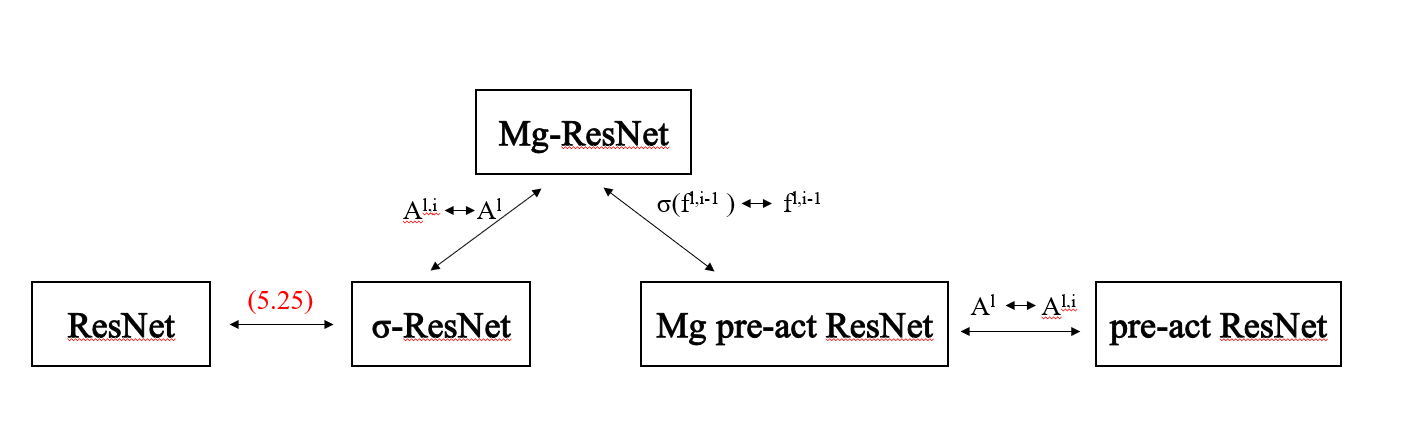
\includegraphics[width=1.0\textwidth]{Mgnetrelation} 
	\end{center}
	%\caption{Connections}
	\label{fig:mgnet}
\end{figure}
\vspace{-26pt}
%Because of the linearity of $\xi^{\ell,i}$, the above forms of iResNet and ResNet
%are equivalent to the previous as \eqref{dualmgnet} and \eqref{tilde-resnet}.
In this sense, these MgNet related models can be understood as
 models between pre-act ResNet and ResNet. And all these models can be
 understood as iteration in the data space as a dual relationship with
 feature space as MgNet.
 
 
The rationality of replacing  $A^{\ell,i}$ by layer independent $A^{\ell}$ may
be justified by the following theorem. 
\begin{theorem}\label{thm:CNN}
On each grid $\mathcal T_\ell$, 
\begin{enumerate}
	\item Any CNN model with
%	CNN and Mg-ResNet] 
	\begin{equation}
	\label{CNN1}
	f^{\ell,i} =   \chi^{\ell,i} \circ \sigma (f^{\ell,i-1}),
	\end{equation} 
	can be written as
	\begin{equation}\label{Res-CNN1}
	f^{\ell,i} = \sigma(f^{\ell,i-1}) - \xi^{\ell} \circ \sigma \circ \eta^{\ell,i} \circ\sigma ( f^{\ell,i-1}).
	\end{equation}
	\item Any CNN model with 
%	[CNN and ResNet] 
	\begin{equation}
	\label{CNN2}
	f^{\ell,i} =   \sigma\circ\chi^{\ell,i} (f^{\ell,i-1}).
	\end{equation}
	can be written as 
	\begin{equation}\label{Res-CNN2}
	f^{\ell,i} = \sigma\left(f^{\ell,i-1} - \xi^{\ell} \circ \sigma \circ \eta^{\ell,i}  ( f^{\ell,i-1})\right).
	\end{equation}
\end{enumerate}

%\begin{equation}
% \chi^{\ell,i}: \mathbb{R}^{n_\ell \times n_\ell \times c_\ell} 
% \mapsto \mathbb{R}^{n_\ell \times n_\ell \times c_\ell},
%\end{equation}
\end{theorem}
\begin{proof}
%	Without loss of generality, consider the classical CNN with 
%	\begin{equation}
%	f^{\ell,i} =   ({\rm id}  + \tilde \eta^{\ell,i} )\circ \sigma (f^{\ell,i-1}).
%	\end{equation}
Let use prove the first case as an example, 
the second case can be proven with the same process.

With similar structure in MgNet, we can take
\begin{equation}
\label{xi-cnn1}
\xi^{\ell}= \hat \delta^\ell :=  [\hat \delta_1, \cdots, \hat \delta_{{c_\ell}}],
\end{equation}
and 
\begin{equation}
\label{eta-ell}
\eta^{\ell,i} = [{\rm id}_{c_\ell}, -{\rm id}_{c_\ell}] \circ (\chi^{\ell,i} - {\rm id}_{c_\ell}).
\end{equation}
Here 
\begin{equation}
{\rm id}_{c_\ell}: \mathbb{R}^{n_\ell \times n_\ell \times c_\ell} 
\mapsto \mathbb{R}^{n_\ell \times n_\ell \times c_\ell},
\end{equation}
is the identity map and 
\begin{equation}
\hat \delta_k :  \mathbb{R}^{n_\ell \times n_\ell \times 2c_\ell} 
\mapsto \mathbb{R}^{n_\ell \times n_\ell},
\end{equation}
with 
\begin{equation}\label{eq:hatdelta}
\hat \delta_k([X ,Y]) = -([X]_k + [Y]_k),
\end{equation}
for any $X, Y \in \mathbb{R}^{n_\ell \times n_\ell \times c_\ell}$ 
and $[X,Y] \in \mathbb{R}^{n_\ell \times n_\ell \times 2c_\ell} $.


	First, we see that $\eta^{\ell,i}$ with the above 
	form is a convolution from $\mathbb{R}^{n_\ell \times n_\ell \times c_\ell}$
	to  $\mathbb{R}^{n_\ell \times n_\ell \times 2c_\ell}$.
	Following the identity
	\begin{equation}
	ReLU(x) + ReLU(-x) = x,
	\end{equation}
	and the definition of $\xi^{\ell}$ i.e. 
	\begin{equation}
	\xi^{\ell} = \hat \delta^\ell,
	\end{equation}
	as a special case in MgNet. 
	For more details, we can give a exact form of 
	$\hat \delta_k$ as in \eqref{eq:hatdelta} with
	\begin{equation}
	\hat \delta_k = [0, \cdots,0, -\delta, \cdots 0;  0, \cdots,0, -\delta, \cdots 0],  \quad k = 1:{c_\ell},
	\end{equation}
	where $\delta$ is the identity kernel during one channel.
	
	At last, we have
	\begin{align}
	\left[\xi^{\ell} \circ \sigma \circ [{\rm id}_{c_\ell}, -{\rm id}_{c_\ell}] (x) \right]_k &=  \left[\xi^{\ell} \circ \sigma \circ [x, -x]  \right]_k, \\
	&= \hat \delta_k ( [\sigma(x), \sigma(-x)]),  \\
	&= -\delta([\sigma(x)]_k) - \delta([\sigma(-x)]_k),\\
	&=-( \sigma([x]_k)+ \sigma(-[x]_k)) , \\
	&=  -[x]_k
	\end{align}
	Thus to say,
	\begin{equation}
	\xi^{\ell} \circ \sigma \circ [{\rm id}_{c_\ell}, -{\rm id}_{c_\ell}]  = -{\rm id}_{c_\ell}.
	\end{equation}
	Then the modified dual form of MgNet in \eqref{tilde-resnet} becomes
	\begin{align}
	f^{\ell,i} &= \sigma(f^{\ell,i-1}) - \xi^{\ell,i} \circ \sigma \circ \eta^{\ell,i} \circ\sigma ( f^{\ell,i-1}) , \\
	&=  \sigma(f^{\ell,i-1}) - \left( \xi^{\ell} \circ \sigma \circ [{\rm id}_{c_\ell}, -{\rm id}_{c_\ell}] \right) 
	\circ (\chi^{\ell,i} - {\rm id}_{c_\ell})\circ \sigma(f^{\ell,i-1})\\
	&=\sigma(f^{\ell,i-1}) + (\chi^{\ell,i} -{\rm id}_{c_\ell})\circ \sigma(f^{\ell,i-1}),  \\
	&=\chi^{\ell,i} \circ  \sigma (f^{\ell,i-1}).
	\end{align}
	This covers \eqref{Res-CNN1}.
\end{proof}


\begin{remark}
Theorems~\ref{thm:CNN} shows that general CNN in
the forms of either \eqref{CNN1} or \eqref{CNN2} can be written recast
as \eqref{Res-CNN1} or \eqref{Res-CNN2} with the data-feature mapping 
$A^\ell=\xi^\ell$ that is not only independent of the layers, but is
actually given a priori as in \eqref{xi-cnn1}.  In
view of Theorems~\ref{thm:mgnet1} and \ref{thm:mgnet2}, the classic
CNN models can be essentially recovered from MgNet by choosing
$\xi^\ell$ a priori as in  \eqref{xi-cnn1}.  Since
the classic CNN models have been extensively tested to be successful,
the more general MgNet with more general $\xi^\ell$ (to be trained)
are expected to be more efficient than the classic CNN models. 
\end{remark}

%At last we have the next relation:
%\input{MgNet-relation.tex}
%\section{Constrained linear data-feature mapping from MgNet to interpret ResNet}
In this section, we will establish a new understanding of pre-act ResNet  
by involving the idea that the pre-act ResNet block is an iterative scheme for solving some 
hidden model in each grid, which is also the fundamental assumption in MgNet. 
More details about this mathematical interpreting model for CNN can be found
in~\cite{he2019constrained}.

The main point here is the introduction of 
the so-called data and feature space for CNN, which is analogous to the 
function space and its duality in the theory of multigrid 
methods~\cite{xu2017algebraic}. 
Namely, following~\cite{he2019mgnet} we introduce 
the next data-feature mapping model in every grid level follows:
\begin{equation}\label{eq:fmapping}
A^{\ell} \ast u^\ell = f^{\ell},
\end{equation}
where $f^\ell$ and $u^\ell$ belong to the data and feature space at $\ell$-th grid. 
We now make the following two important observations for this data-feature mapping:
\begin{itemize}
	\item The mapping in \eqref{eq:fmapping} is linear, more specifically it is just a convolution with multichannel, zero
	padding and stride one as in pre-act ResNet.
	\item In each level, namely between two consecutive pooling, there is only one
	data-feature mapping, or we say that $A^\ell$ only depends on $\ell$, but not on number of layers.
\end{itemize}
We note that the assumption that these linear data-feature mapping
depend only on the grid level $\ell$ is motivated from a basic property of 
multigrid methods~\cite{xu1992iterative, hackbusch2013multi, xu2017algebraic}.

Besides \eqref{eq:fmapping}, we introducing an important constrained condition
in feature space that
\begin{equation}\label{eq:positive}
u^{\ell,i} \ge 0.
\end{equation}
The rationality of this constraint in feature space can be interpreted as follows.
First of all, from the real neural system, the real neurons will only be
active if the electric signal is greater than certain thresholding value. 
Namely, we can think that human brains can only see features 
with certain threshold.
On the other hand, the ``shift'' invariant property of feature space in CNNs,
namely, $u+a$ will not change the classification results. This means that $u+a$ should
have the same classification result with $u$. That is to say, we may assume that
$u \ge 0$ to reduce some redundancy of $u$.

Based on these assumptions above, what we need to do next is to
solve the data-feature mapping equation in \eqref{eq:fmapping}.
We will adopt some classical iterative methods~\cite{xu1992iterative} in scientific computing
to solve the system \eqref{eq:fmapping} and obtain that 
\begin{equation}\label{BAmapping}
u^{\ell,i} = u^{\ell,i-1} + B^{\ell,i} \ast (f^{\ell} - A^{\ell}\ast u^{\ell,i-1}),~ i = 1:\nu_\ell,
\end{equation}
where $u^{\ell} \approx u^{\ell,\nu_\ell}$. 
For more details about iterative methods
in numerical analysis, we refer to~\cite{xu1992iterative, hackbusch1994iterative, golub2012matrix}.
To preserve \eqref{eq:positive}, we naturally use the ReLU activation function $\sigma$
to modify \eqref{BAmapping} as follows
\begin{equation}
\label{eq:uBfAu}
u^{\ell,i} = u^{\ell,i-1} + \sigma \circ B^{\ell,i}\ast \sigma  (f^\ell -  A^\ell
\ast u^{\ell,i-1}), \quad i=1:\nu_\ell,
\end{equation}
which leads the the basic iterative scheme in MgNet.

Now, let us consider the iteration for residual. Because of the linearity of convolution in data-feature mapping,
if we consider the residual $r^{\ell,j} = f^{\ell} - A^{\ell}\ast u^{\ell,j}$, 
\eqref{eq:uBfAu} leads to the next iterative forms for residuals
\begin{equation}\label{eq:pre-actResNet_residual}
r^{\ell, i} = r^{\ell,i-1} - A^\ell \ast \sigma \circ B^{\ell,i}\ast \sigma(r^{\ell,i-1}).
\end{equation}
This is the same as \eqref{eq:pre-act ResNet} under the constraint $A^{\ell,i} = A^{\ell}$ in pre-act ResNet.

We summarize the above derivation in the following simple theorem.
\begin{theorem}\label{thm:1} Under the assumption that there is only
	one linear data-feature mapping in each grid $\ell$, i.e. $A^{\ell,i} = A^{\ell}$, 
	the iterative form in feature space as in \eqref{BAmapping} is equivalent to 
	\eqref{eq:pre-actResNet_residual} if $A^\ell$ is invertible where $r^{\ell,i} = f^\ell - A^{\ell}\ast u^{\ell,i}$.
\end{theorem}



%%%%%%%%%%%%%%%%%%%%%%%%%%%%%%%%%%%%%%%%%%%%




\bibliographystyle{abbrv}\bibliography{ref,ref_mgcnn,../3FEM/3FEM}

\end{document}


